\subsubsection{SVM Results}
After implementing the methodology described earlier, it was found that the best hyperparameter was a penalty for misclassification of 1 (C) and a Radial Basis Function (RBF) as kernel. With the previous hyperparameters, the model achieved an accuracy of 0.87. 
Table~\ref{tab:gru_classification_report} shows the classification report. As seen, the highest metric is the Recall for Non-toxic messages. This suggests that the model is more likely to correctly identify non-toxic comments and can have some struggles to capture all true positives in the toxic class. Although the precision for the positive class is high (0.91), indicating that when the model predicts toxicity it is usually correct, the lower recall reveals that some toxic instances are being misclassified as non-toxic. The results are similar to the XGBoostClassifier, indicating that this model could also benefit with more toxic examples.

\begin{table}[H]
    \centering
    \caption{Classification report of the SVM model}
    \label{tab:gru_classification_report}
    \begin{tabular}{lcccc}
        \toprule
        Class & Precision & Recall & F1-score & Support \\
        \midrule
        0 (No Hate Speech) & 0.83 & 0.91 & 0.87 & 4626 \\
        1 (Hate Speech)    & 0.91 & 0.83 & 0.86 & 4912 \\
        \midrule
        Accuracy           & \multicolumn{4}{c}{0.87 (on 9538 samples)} \\
        Macro Avg          & 0.87 & 0.87 & 0.87 & 9538 \\
        Weighted Avg       & 0.87 & 0.87 & 0.87 & 9538 \\
        \bottomrule
    \end{tabular}
\end{table}

In Figure~\ref{fig:confusion_matrix_svm}, the confusion matrix can be seen, which reflects the quality of the model. There are over 1200 examples that were misclassified, showing that there is room for improvement for this model. In particular, there are more toxic comments that are not recognized correctly.

\begin{figure}[H]
    \centering
    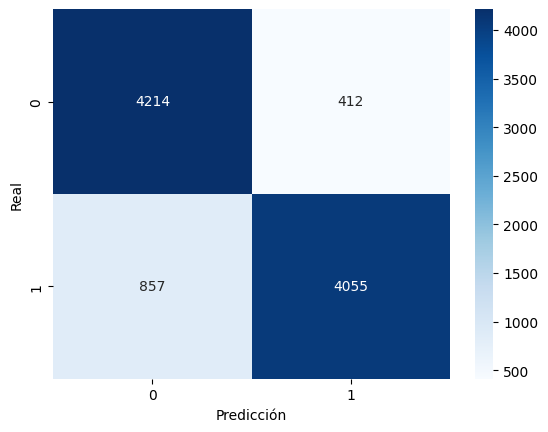
\includegraphics[width=\linewidth]{images/ConfusionMatrixSVMTestSet.png}
    \caption{Confusion matrix for the SVM model evaluated on the test set.}
    \label{fig:confusion_matrix_svm}
\end{figure}